\documentclass[tikz,border=3pt]{standalone}
\usepackage[utf8]{inputenc}
\usepackage[T1]{fontenc}
\usepackage{lmodern}
\renewcommand{\familydefault}{\sfdefault}
\usepackage{sansmath}\sansmath
\usepackage{pgfplots}\pgfplotsset{compat=1.18,/pgf/number format/use comma,/pgf/number format/1000 sep={.}}
\usetikzlibrary{arrows.meta,calc,positioning,decorations.pathmorphing,patterns}
% paleta del sitio
\definecolor{nar}{HTML}{E8680C}\definecolor{narc}{HTML}{FFB35C}\definecolor{hielo}{HTML}{FFF3E8}
\definecolor{tinta}{HTML}{1D1D1F}\definecolor{gris}{HTML}{6E6E73}\definecolor{lila}{HTML}{7C5CF0}
\definecolor{azul}{HTML}{2F6FD6}\definecolor{menta}{HTML}{17A673}\definecolor{coral}{HTML}{E8342A}
\begin{document}
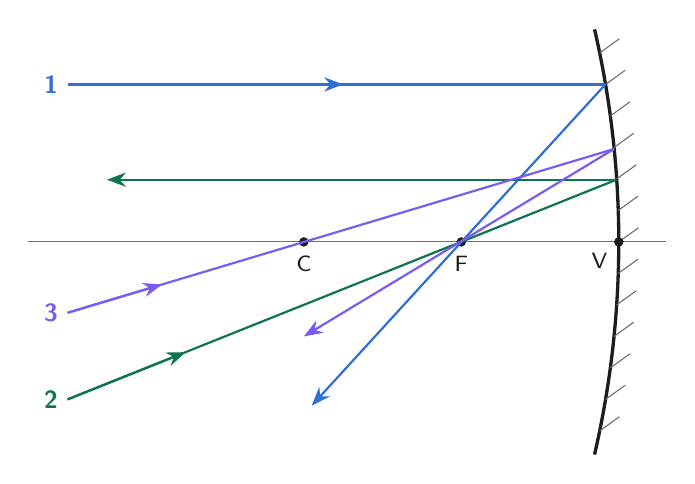
\begin{tikzpicture}[font=\footnotesize,>={Stealth[length=2.4mm]}]
\draw[gris] (-7.5,0) -- (0.6,0);
\draw[very thick,tinta,domain=-2.7:2.7,samples=60,smooth] plot ({-12+sqrt(144-\x*\x)},\x);
\foreach \y in {-2.4,-2.0,...,2.41} \draw[gris,thin] ({-12+sqrt(144-\y*\y)},\y) -- ++(0.25,0.18);
\foreach \x/\t in {-2/F,-4/C} {\fill[tinta] (\x,0) circle (0.06); \node[below,text=tinta] at (\x,-0.05) {\t};}
\fill[tinta] (0,0) circle (0.06); \node[below left,text=tinta] at (-0.02,-0.02) {V};

\draw[azul,thick] (-7,2.0) -- (-0.17,2.0); \draw[->,azul,thick] (-7,2.0) -- (-3.5,2.0);
\draw[->,azul,thick] (-0.17,2.0) -- (-3.9,-2.08);
\node[left,font=\small\bfseries,text=azul] at (-7,2.0) {1};
\draw[menta!70!black,thick] (-7,-2.0) -- (-0.03,0.79); \draw[->,menta!70!black,thick] (-7,-2.0) -- (-5.5,-1.4);
\draw[->,menta!70!black,thick] (-0.03,0.79) -- (-6.5,0.79);
\node[left,font=\small\bfseries,text=menta!70!black] at (-7,-2.0) {2};
\draw[lila,thick] (-7,-0.9) -- (-0.06,1.18); \draw[->,lila,thick] (-7,-0.9) -- (-5.8,-0.54);
\draw[->,lila,thick] (-0.06,1.18) -- (-4,-1.2);
\node[left,font=\small\bfseries,text=lila] at (-7,-0.9) {3};
\end{tikzpicture}
\end{document}
